\documentclass[10pt,letterpaper]{article}
\usepackage{fontspec}
\usepackage{amsmath,amssymb}
\usepackage{graphicx}
\usepackage{xcolor}
\usepackage{tcolorbox}
\tcbuselibrary{skins}
\usepackage{geometry}
\usepackage{booktabs}
\usepackage{colortbl}
\usepackage{fancyhdr}
\usepackage{titlesec}
\usepackage[shortlabels,inline]{enumitem}
\usepackage{tabularx}
\usepackage{array}
\usepackage{multicol}
\usepackage{tikz}

\setmainfont{Times New Roman}
\setsansfont{Arial}

\geometry{
    paperwidth=612.05pt,
    paperheight=720.05pt,
    top=20pt,
    headheight=14pt,
    headsep=12pt,
    bottom=28pt,
    footskip=12pt,
    left=36pt,
    right=36pt
}

\definecolor{stewartcyan}{RGB}{0, 118, 186}
\definecolor{stewartred}{RGB}{218, 41, 28}
\definecolor{stewarttableheader}{RGB}{210, 224, 238}
\definecolor{stewarttablehead}{RGB}{210, 224, 238}
\definecolor{tableblue}{RGB}{210, 224, 238}
\definecolor{stewartlightblue}{RGB}{235, 243, 250}
\definecolor{stewartblue}{RGB}{0, 118, 186}
\definecolor{stewartgray}{RGB}{120, 120, 120}
\definecolor{stewartlightgray}{RGB}{240, 240, 240}
\definecolor{stewartpurple}{RGB}{85, 30, 95}
\definecolor{stewartpurplebg}{RGB}{243, 238, 245}
\definecolor{stewartpurpletext}{RGB}{85, 30, 95}
\definecolor{darkgray}{RGB}{40, 40, 40}

\pagestyle{fancy}
\fancyhf{}
\renewcommand{\headrulewidth}{0pt}

\providecommand{\makecell}[2][c]{\begin{tabular}[#1]{@{}c@{}}#2\end{tabular}}
\providecommand{\faDesktop}{\textbf{[Máy tính]}}
\providecommand{\casicon}{\textbf{\textsf{[CAS]}}}
\providecommand{\ticon}{\textbf{\textsf{[T]}}}
\providecommand{\captionof}[2]{\par\vspace{2pt}{\small\textbf{#1}: #2}\par}
\NewDocumentEnvironment{tasks}{o d()}{\begin{enumerate}}{\end{enumerate}}
\providecommand{\task}{\item}
\newenvironment{redframebox}{\begin{definitionbox}}{\end{definitionbox}}

\newtcolorbox{definitionbox}{
    colback=white,
    colframe=stewartred,
    arc=0mm,
    boxrule=0.9pt,
    left=3.5mm, right=3.5mm, top=3mm, bottom=3mm
}

\begin{document}

\begin{document}
\noindent
\begin{minipage}[t]{0.48\textwidth}
Bệnh viện Đại học thuộc Đại học Nam California tại Los Angeles. Hãy sử dụng đồ thị đó để ước lượng tập giá trị của hàm gia tốc nền thẳng đứng tại USC trong trận động đất Northridge.

\vspace{0.4em}
\textbf{6.} Trong mục này, chúng ta đã thảo luận các ví dụ về những hàm số thông thường trong đời sống hàng ngày: dân số là hàm số của thời gian, cước phí bưu chính là hàm số của khối lượng bưu kiện, nhiệt độ nước là hàm số của thời gian. Hãy đưa ra ba ví dụ khác về hàm số từ đời sống thường ngày được mô tả bằng lời. Bạn có thể nói gì về tập xác định và tập giá trị của từng hàm số đó? Nếu có thể, hãy vẽ phác thảo đồ thị của mỗi hàm số.

\vspace{0.45em}
\textbf{\textsf{\color{stewartcyan}7--14}}\quad Xác định xem phương trình hoặc bảng giá trị đã cho có xác định $y$ là một hàm số của $x$ hay không.

\vspace{0.3em}
\begin{tabular}{@{}p{0.48\linewidth}@{\hspace{0.04\linewidth}}p{0.48\linewidth}@{}}
\textbf{7.} $3x - 5y = 7$ & \textbf{8.} $3x^2 - 2y = 5$ \\[0.45em]
\textbf{9.} $x^2 + (y - 3)^2 = 5$ & \textbf{10.} $2xy + 5y^2 = 4$ \\[0.45em]
\textbf{11.} $(y + 3)^3 + 1 = 2x$ & \textbf{12.} $2x - |y| = 0$
\end{tabular}

\vspace{0.45em}
\noindent
\begin{minipage}[t]{0.48\linewidth}
\setlength{\tabcolsep}{3pt}
\renewcommand{\arraystretch}{1.15}
\textbf{13.}\hspace{0.3em}
\begin{tabular}[t]{|c|c|}
\hline
\rowcolor{tableblue} $x$ & $y$ \\
\rowcolor{tableblue} Chiều cao (in) & Cỡ giày \\
\hline
72 & 12 \\
60 & 8 \\
60 & 7 \\
63 & 9 \\
70 & 10 \\
\hline
\end{tabular}
\end{minipage}%
\hfill
\begin{minipage}[t]{0.50\linewidth}
\setlength{\tabcolsep}{3pt}
\renewcommand{\arraystretch}{1.15}
\textbf{14.}\hspace{0.3em}
\begin{tabular}[t]{|c|c|}
\hline
\rowcolor{tableblue} $x$ & $y$ \\
\rowcolor{tableblue} Năm & Học phí (\$) \\
\hline
2016 & 10{,}900 \\
2017 & 11{,}000 \\
2018 & 11{,}200 \\
2019 & 11{,}200 \\
2020 & 11{,}300 \\
\hline
\end{tabular}
\end{minipage}

\vspace{0.55em}
{\color{stewartcyan}\hrule height 0.6pt}
\vspace{0.55em}

\textbf{\textsf{\color{stewartcyan}15--18}}\quad Xác định xem đường cong đã cho có phải là đồ thị của một hàm số của $x$ hay không. Nếu phải, hãy nêu rõ tập xác định và tập giá trị của hàm số đó.

\vspace{0.4em}
\noindent
\begin{minipage}[t]{0.48\linewidth}
    \textbf{15.}\\[0.2em]
    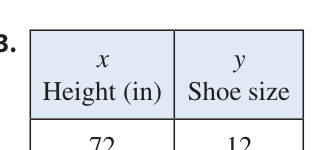
\includegraphics[width=0.95\linewidth]{images/p0053_fig1.png}
\end{minipage}%
\hfill
\begin{minipage}[t]{0.48\linewidth}
    \textbf{16.}\\[0.2em]
    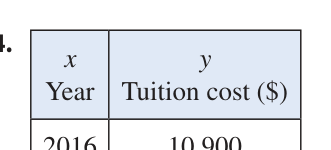
\includegraphics[width=0.95\linewidth]{images/p0053_fig2.png}
\end{minipage}

\vspace{0.5em}
\noindent
\begin{minipage}[t]{0.48\linewidth}
    \textbf{17.}\\[0.2em]
    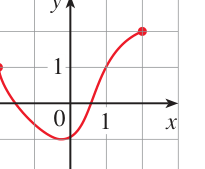
\includegraphics[width=0.95\linewidth]{images/p0053_fig3.png}
\end{minipage}%
\hfill
\begin{minipage}[t]{0.48\linewidth}
    \textbf{18.}\\[0.2em]
    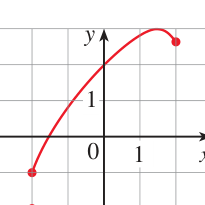
\includegraphics[width=0.95\linewidth]{images/p0053_fig4.png}
\end{minipage}

\vspace{0.55em}
{\color{stewartcyan}\hrule height 0.6pt}
\vspace{0.55em}

\textbf{19.} Hình bên là đồ thị nhiệt độ trung bình toàn cầu $T$ trong thế kỷ 20. Hãy ước lượng các giá trị sau:
\begin{enumerate}[label=(\alph*), itemsep=1pt, topsep=2pt, leftmargin=1.5em]
    \item Nhiệt độ trung bình toàn cầu vào năm 1950
    \item Năm mà nhiệt độ trung bình đạt $14{,}2^\circ\text{C}$
\end{enumerate}
\end{minipage}%
\hfill
\begin{minipage}[t]{0.48\textwidth}
\begin{enumerate}[label=(\alph*), itemsep=1pt, topsep=0pt, leftmargin=1.5em]
    \setcounter{enumi}{2}
    \item Các năm mà nhiệt độ đạt giá trị nhỏ nhất và lớn nhất
    \item Tập giá trị của $T$
\end{enumerate}

\begin{center}
    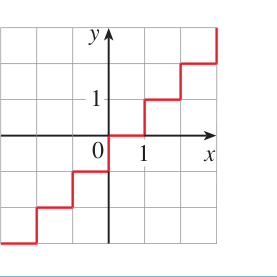
\includegraphics[width=0.78\linewidth]{images/p0053_fig5.png}
\end{center}
\vspace{-0.5em}
{\footnotesize \textit{Nguồn:} Phỏng theo \textit{Globe and Mail} [Toronto], 5 tháng 12 năm 2009. Bản in.}

\vspace{0.5em}
\textbf{20.} Cây cối sinh trưởng nhanh hơn và tạo các vòng gỗ rộng hơn vào những năm ấm áp, đồng thời sinh trưởng chậm hơn và tạo các vòng gỗ hẹp hơn vào những năm mát mẻ hơn. Đồ thị bên thể hiện độ rộng vòng gỗ của một cây thông Siberi từ năm 1500 đến năm 2000.
\begin{enumerate}[label=(\alph*), itemsep=1pt, topsep=2pt, leftmargin=1.5em]
    \item Tập giá trị của hàm độ rộng vòng gỗ là gì?
    \item Đồ thị có xu hướng cho biết điều gì về nhiệt độ của Trái Đất? Đồ thị có phản ánh các vụ phun trào núi lửa vào giữa thế kỷ 19 không?
\end{enumerate}

\begin{center}
    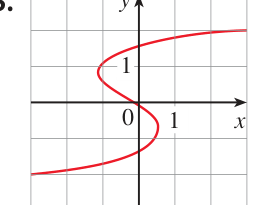
\includegraphics[width=0.82\linewidth]{images/p0053_fig6.png}
\end{center}
\vspace{-0.5em}
{\footnotesize \textit{Nguồn:} Phỏng theo G. Jacoby và cộng sự, “Mongolian Tree Rings and 20th-Century Warming,” \textit{Science} 273 (1996): 771--73.}

\vspace{0.5em}
\textbf{21.} Bạn bỏ vài viên đá lạnh vào một cốc thủy tinh, rót đầy nước lạnh vào cốc, sau đó để cốc nằm yên trên bàn. Hãy mô tả nhiệt độ của nước thay đổi như thế nào theo thời gian trôi qua. Sau đó vẽ phác thảo đồ thị nhiệt độ của nước như một hàm số của thời gian trôi qua.

\vspace{0.4em}
\textbf{22.} Bạn đặt một chiếc bánh đông lạnh vào lò nướng và nướng trong một giờ. Sau đó bạn lấy bánh ra và để nguội. Hãy mô tả nhiệt độ của bánh thay đổi như thế nào theo thời gian trôi qua. Sau đó vẽ phác thảo đồ thị nhiệt độ của chiếc bánh như một hàm số của thời gian.

\vspace{0.4em}
\textbf{23.} Đồ thị thể hiện mức tiêu thụ điện năng trong một ngày vào tháng Chín tại San Francisco ($P$ được đo bằng megawatt; $t$ được đo bằng giờ tính từ nửa đêm).
\begin{enumerate}[label=(\alph*), itemsep=1pt, topsep=2pt, leftmargin=1.5em]
    \item Mức tiêu thụ điện năng vào lúc 6 giờ sáng là bao nhiêu? Vào lúc 6 giờ tối là bao nhiêu?
\end{enumerate}
\end{minipage}
\end{document}
